\subsection{Reticolazione covalente via alcossiammine}
\begin{frame}\frametitle{Reticolazione covalente via alcossiammine}
I polimeri che si basano su interazioni \textbf{non covalenti subiscono deformazioni} permanenti, quelli basati su interazioni \textbf{covalenti diventano dinamici solo se scaldati}.

Nel sistema in figura i \textbf{radicali} formati sono \textbf{stabili} e non reagiscono con altri gruppi funzionali presenti.

Il sistema può essere \textbf{de-reticolato} a caldo in presenza di un \textbf{eccesso di alcossiammina}.
\begin{figure}{\centering{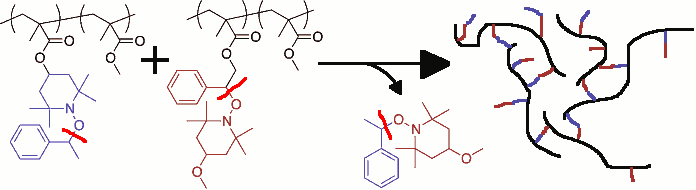
\includegraphics[width=0.9\textwidth]{covalente/alcossiammina.png}}}\end{figure}\vspace{-20pt}
\footnote{\tiny  \fullcite{radicali}}
\end{frame}

\subsection{Reticolazione covalente via Diels Alder}
\begin{frame}\frametitle{Reticolazione covalente via Diels Alder}
\begin{columns}
 \column{0.6\linewidth}
Con la reticolazione covalente reversibile si possono avere \textbf{a temperatura ambiente le proprietà di un termoindurente} (alto modulo elastico, \textbf{1}) \textbf{oppure dinamici a temperatura ambiente} (\textbf{3}). Possono essere in \textbf{singolo componente per evitare lo smescolamento} (\textbf{2}).\vspace{25pt}
\column{0.4\linewidth}\vspace{-10pt}
\begin{figure}{\centering{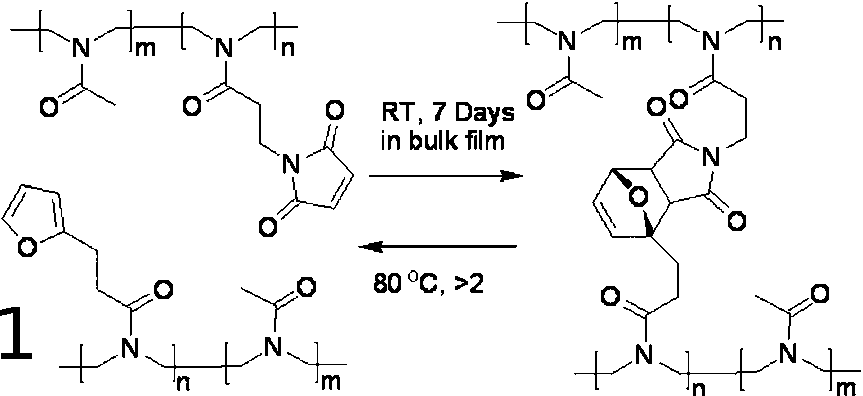
\includegraphics[width=1\textwidth]{covalente/DA.png}}}\end{figure}\vspace{-15pt}
\begin{figure}{\centering{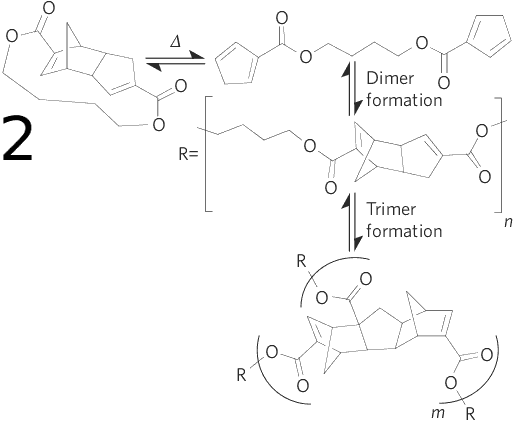
\includegraphics[width=1\textwidth]{covalente/diels-alder1.png}}}\end{figure}

\end{columns}
\vspace{-35pt}
{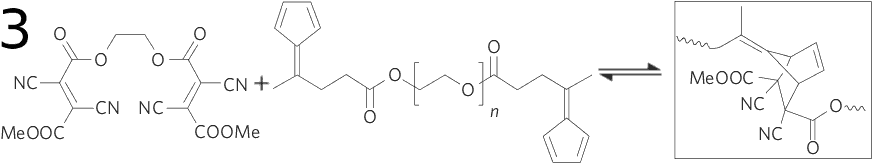
\includegraphics[width=0.8\textwidth]{covalente/diels-alder3.png}}
\footnote{\tiny \leading{3pt} \textbf{1} \fullcite{dielsalder} \textbf{2} \fullcite{dielsalder-dyn} \textbf{3} \fullcite{dielsalder-ram}}

\end{frame}



\subsection{Reticolazione covalente via transesterificazione}
\begin{frame}\frametitle{Reticolazione covalente via transesterificazione}
Questo sistema (a differenza dei precedenti) non si basa su un equilibrio ma su \textbf{reazioni di scambio}, transesterificazioni, dunque \textbf{non sarà disturbato dai solventi}.
Alzando la temperatura, il sistema \textbf{diminuisce in modo graduale la viscosità} passando da solido a fluido viscoso.

La cinetica può essere accelerata introducendo \textbf{catalizzatori inorganici}.
\begin{columns}
 \column{0.8\linewidth}
\begin{figure}{\centering{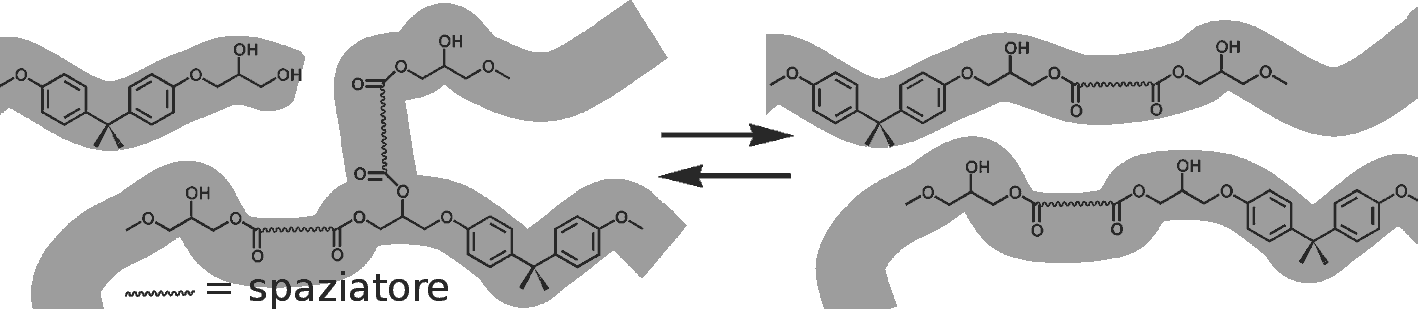
\includegraphics[width=1\textwidth]{covalente/transesterificazione.png}}}\end{figure}
\column{0.2\linewidth}
\begin{figure}{\centering{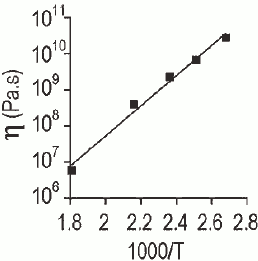
\includegraphics[width=1\textwidth]{covalente/transesterificazione-viscosita.png}}}\end{figure}
\end{columns}
\footnote{\tiny \fullcite{transesterificazione}}
\end{frame}

\subsection{Altro}
\begin{frame}\frametitle{Altro}
\vspace{-5pt}
Molti altri sistemi non sono stati trattati, ad esempio:\vspace{-10pt}
\begin{columns}
 \column{0.5\linewidth}
\begin{figure}{\centering{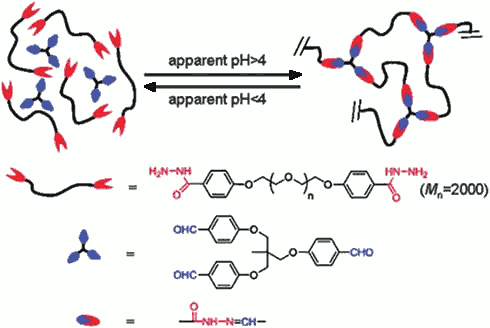
\includegraphics[width=1\textwidth]{covalente/altri-acilidrazone.png}}\\è dinamico}\end{figure}
\vspace{-10pt}\begin{figure}{\centering{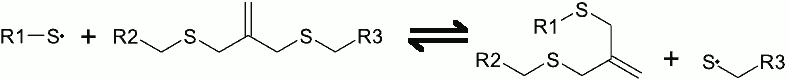
\includegraphics[width=1\textwidth]{covalente/altri-tio.png}}\\la plasticità è fotoindotta}\end{figure}

\column{0.5\linewidth}
\begin{figure}{\centering{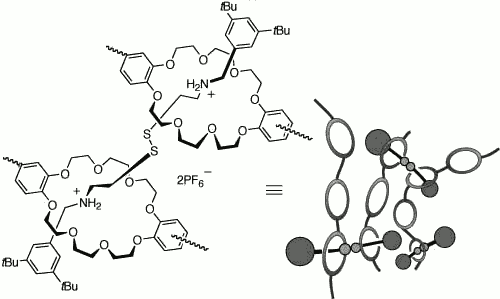
\includegraphics[width=1\textwidth]{covalente/altri-disolf.png}}\\tioli catalizzano l'apertura}\end{figure}

\begin{figure}{\centering{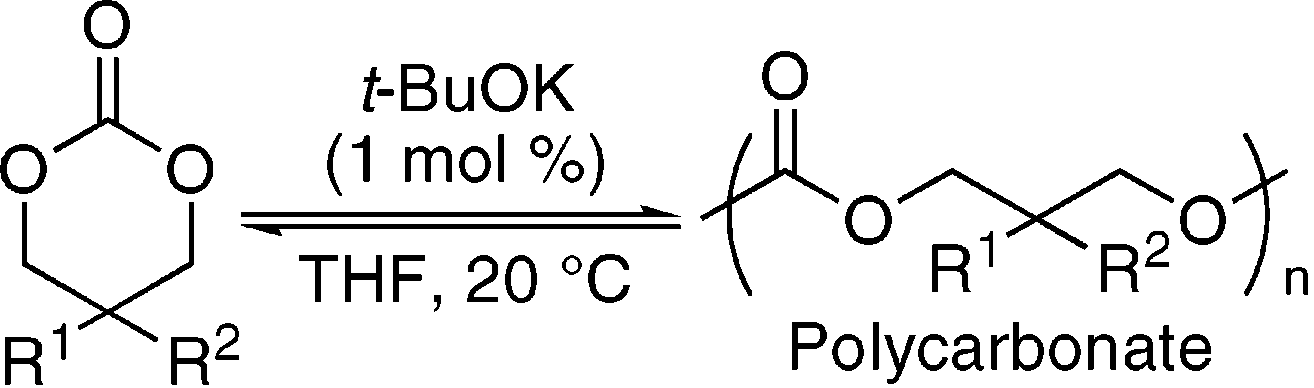
\includegraphics[width=0.7\textwidth]{covalente/altri-carbonato.png}}}\end{figure}

\end{columns}

\end{frame}
